\documentclass[aspectratio=169]{beamer}

% 테마 설정
\usetheme{Madrid}
\usecolortheme{whale}

% 패키지
\usepackage{kotex}
\usepackage{amsmath}
\usepackage{amssymb}
\usepackage{graphicx}
\usepackage{booktabs}
\usepackage{tikz}
\usepackage{xcolor}
\usepackage{pifont}
\usepackage{multirow}
\usetikzlibrary{shapes,arrows,positioning,calc}

% 이미지 경로 설정
\graphicspath{{figures/}}

% 수식 명령어
\DeclareMathOperator*{\argmin}{arg\,min}
\DeclareMathOperator*{\argmax}{arg\,max}

% 색상 정의
\definecolor{mainblue}{RGB}{0,82,147}
\definecolor{accentorange}{RGB}{230,126,34}
\definecolor{accentgreen}{RGB}{39,174,96}
\definecolor{lightgray}{RGB}{240,240,240}

% 프레임 번호 표시
\setbeamertemplate{footline}[frame number]

% 제목 정보
\title[MoLE-Flow]{MoLE-Flow: Mixture of LoRA Experts with \\ Normalizing Flow for Continual Anomaly Detection}
\subtitle{지속적 이상 탐지를 위한 LoRA 전문가 혼합 정규화 흐름}
\author{Author Name}
\institute{Institution Name}
\date{\today}

\begin{document}

%===============================================================================
% 제목 슬라이드
%===============================================================================
\begin{frame}
\titlepage
\end{frame}

%===============================================================================
% 목차
%===============================================================================
\begin{frame}{Contents}
\tableofcontents
\end{frame}

%===============================================================================
\section{Introduction}
%===============================================================================

\begin{frame}{Problem: Continual Anomaly Detection}
\begin{columns}
\begin{column}{0.5\textwidth}
\textbf{산업 환경의 현실}
\begin{itemize}
    \item 새로운 제품이 지속적으로 추가됨
    \item 모든 데이터를 저장/재학습하기 어려움
    \item 이전 제품에 대한 성능 유지 필요
\end{itemize}

\vspace{1em}
\textbf{핵심 문제: Catastrophic Forgetting}
\begin{itemize}
    \item 새 작업 학습 시 이전 작업 성능 급감
    \item 기존 방법: 전체 모델 복제 $\rightarrow$ 메모리 비효율
\end{itemize}
\end{column}

\begin{column}{0.5\textwidth}
\centering
\begin{tikzpicture}[scale=0.8]
    % Task boxes
    \node[draw, fill=mainblue!20, minimum width=2cm, minimum height=1cm] (t0) at (0,2) {Task 0};
    \node[draw, fill=mainblue!30, minimum width=2cm, minimum height=1cm] (t1) at (0,0) {Task 1};
    \node[draw, fill=mainblue!40, minimum width=2cm, minimum height=1cm] (t2) at (0,-2) {Task 2};

    % Arrows
    \draw[->, thick] (t0) -- (t1);
    \draw[->, thick] (t1) -- (t2);

    % Performance indicator
    \node[draw, fill=red!30, minimum width=1.5cm] at (3.5,2) {100\%};
    \node[draw, fill=orange!30, minimum width=1.5cm] at (3.5,0) {70\%};
    \node[draw, fill=red!50, minimum width=1.5cm] at (3.5,-2) {40\%};

    \node at (3.5,3) {\small Task 0 성능};
\end{tikzpicture}
\end{column}
\end{columns}
\end{frame}

\begin{frame}{Our Solution: MoLE-Flow}
\begin{block}{핵심 아이디어: Parameter Isolation}
Base 모델은 공유/고정하고, Task-specific 정보는 경량 어댑터에만 저장
\end{block}

\vspace{1em}
\textbf{5가지 핵심 기여:}
\begin{enumerate}
    \item \textcolor{mainblue}{\textbf{MoLE (Mixture of LoRA Experts)}}: NF coupling 블록에 LoRA 적용
    \item \textcolor{mainblue}{\textbf{WhiteningAdapter}}: 작업 간 분포 차이 정렬
    \item \textcolor{mainblue}{\textbf{Deep Invertible Adapter (DIA)}}: 비선형 매니폴드 적응
    \item \textcolor{mainblue}{\textbf{Prototype-based Router}}: Task ID 없이 자동 라우팅
    \item \textcolor{mainblue}{\textbf{Tail-Aware Loss}}: 분포 경계 학습 강화
\end{enumerate}
\end{frame}

%===============================================================================
\section{Overall Architecture}
%===============================================================================

\begin{frame}{Overall Architecture}
\begin{center}
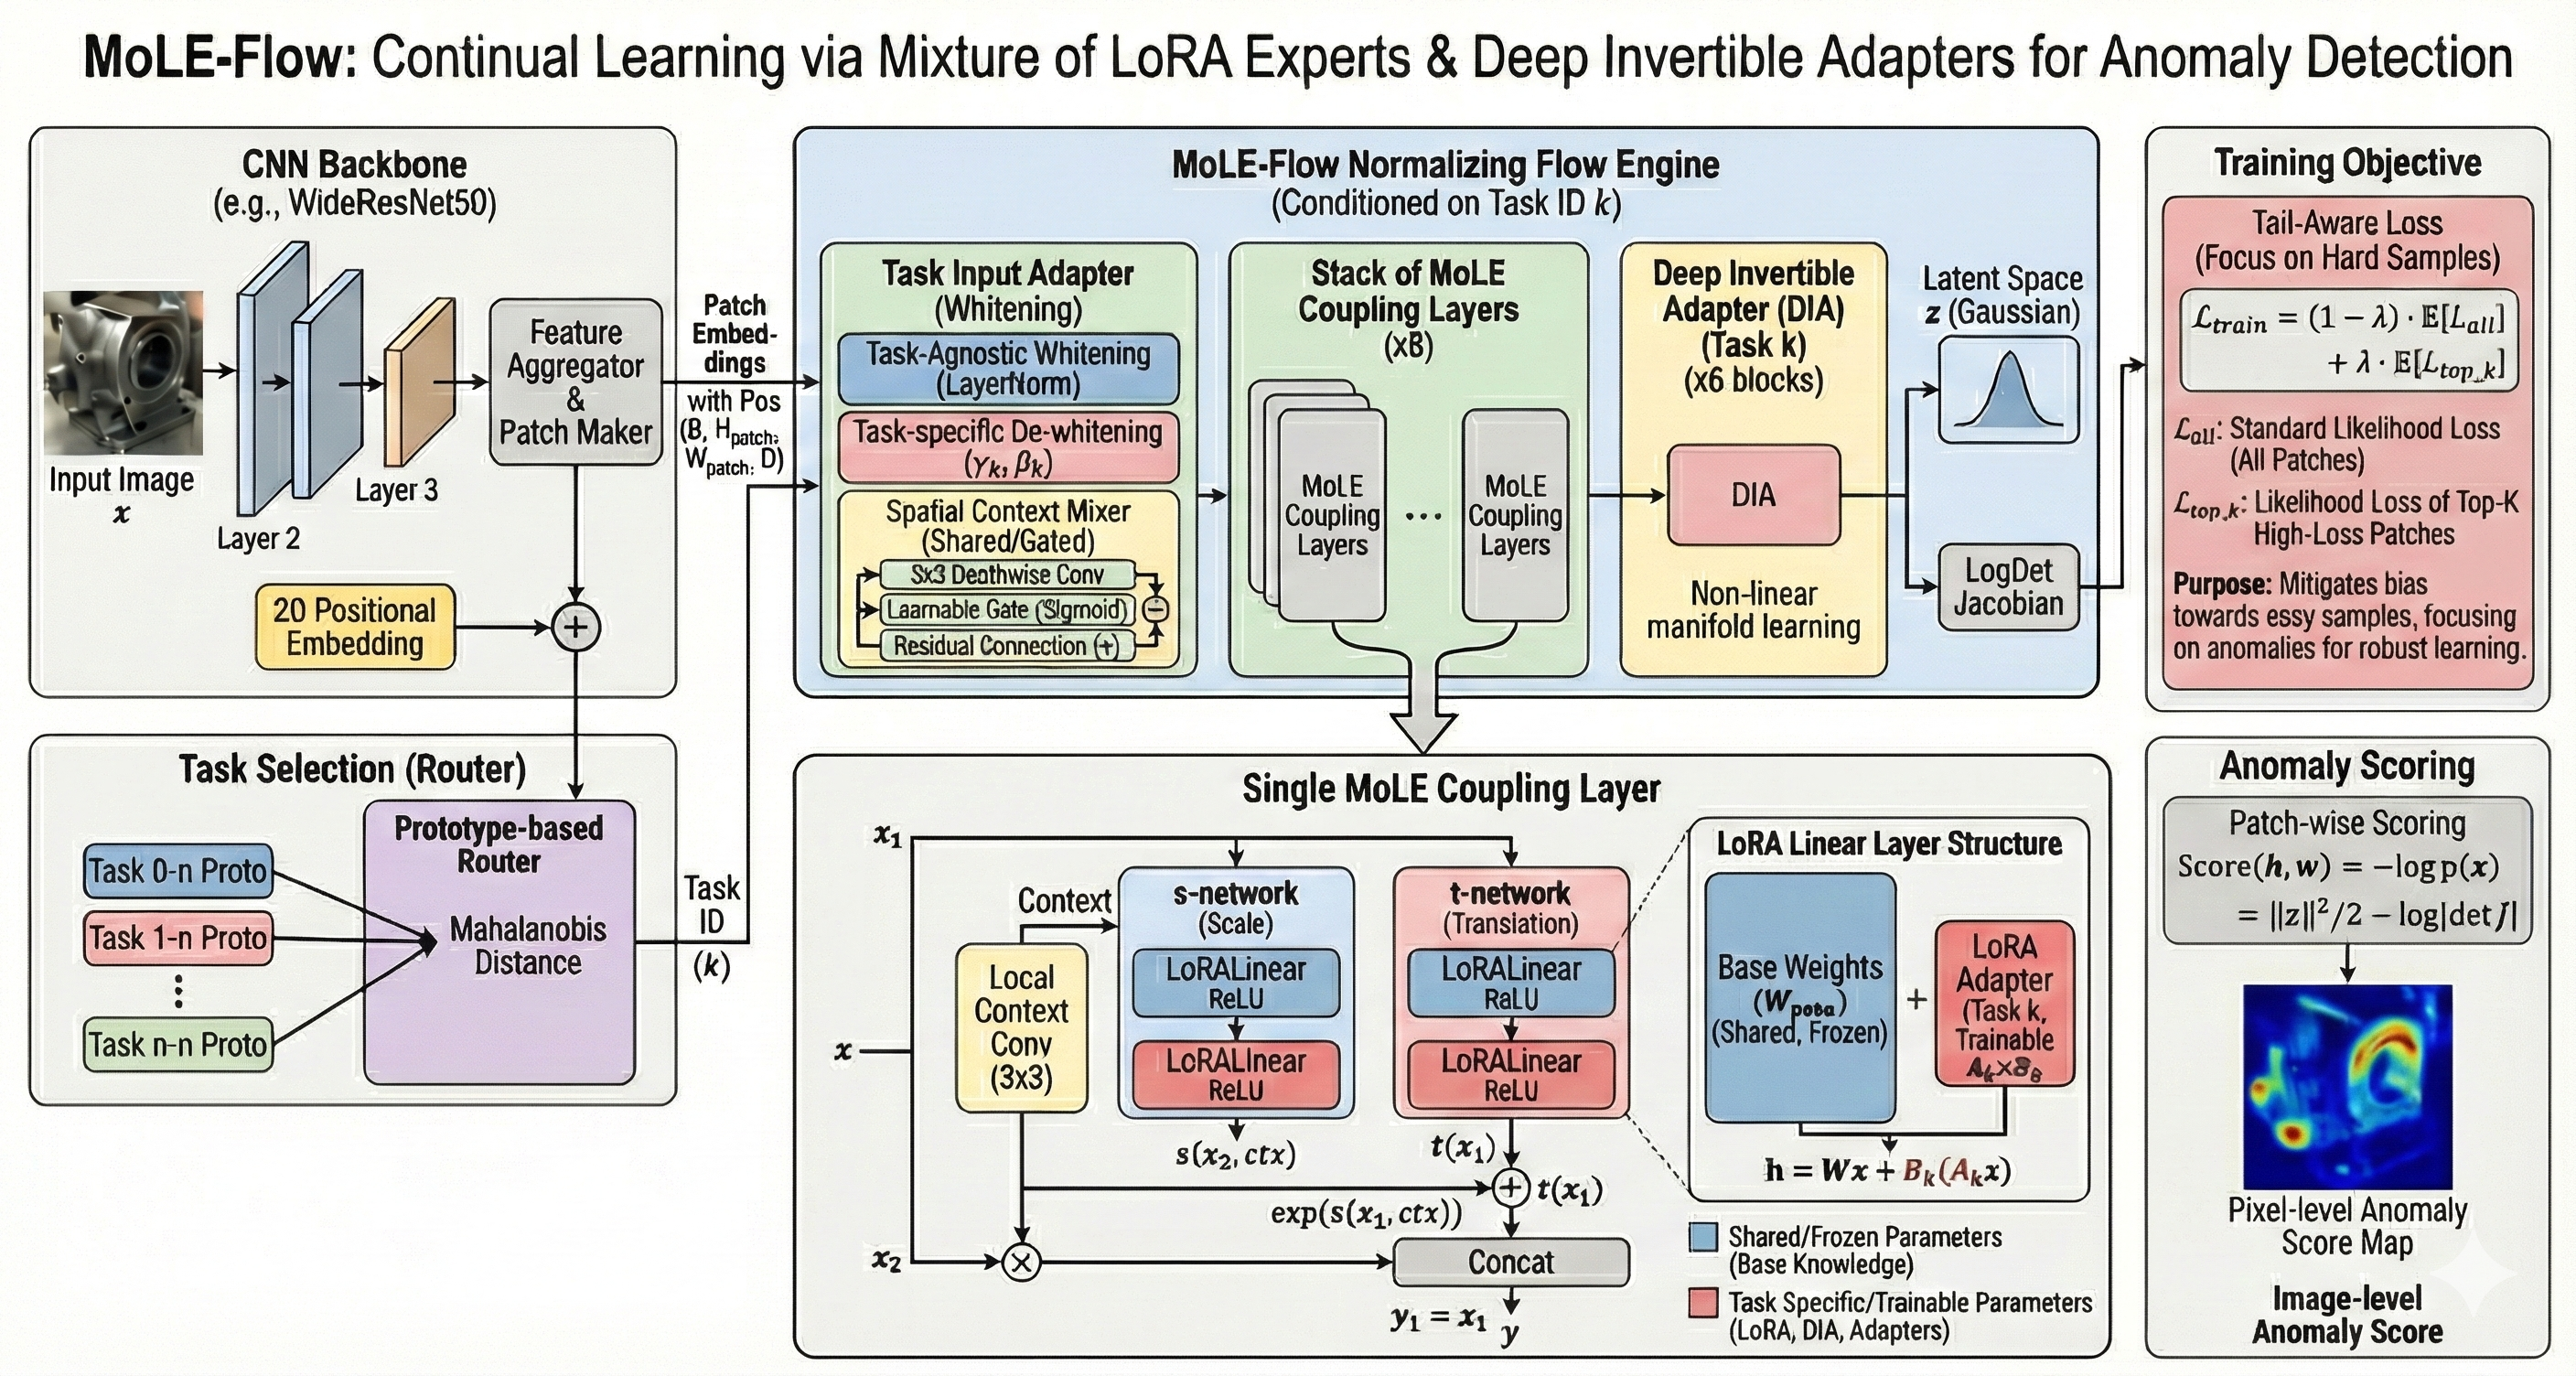
\includegraphics[width=0.95\textwidth]{figures/main2.png}
\end{center}
\end{frame}

\begin{frame}{Overall Architecture - 학습 전략}
\textbf{Parameter Isolation 전략:}
\begin{itemize}
    \item \textcolor{gray}{\textbf{회색 (Shared/Frozen)}}: Backbone, Base NF weights - 모든 작업이 공유
    \item \textcolor{red}{\textbf{빨간색 (Task-specific)}}: LoRA, DIA, Whitening Adapter - 작업별 독립
\end{itemize}

\vspace{1em}
\textbf{학습 전략:}
\begin{itemize}
    \item \textbf{Task 0}: Base NF + 모든 어댑터 학습 $\rightarrow$ Base 동결
    \item \textbf{Task $t > 0$}: 새로운 어댑터(LoRA, Whitening, DIA)만 학습
\end{itemize}

\vspace{1em}
\begin{alertblock}{핵심 장점}
작업당 \textbf{약 10.8\%}의 추가 파라미터만으로 완전한 작업 분리 달성
\end{alertblock}
\end{frame}

\begin{frame}{Detailed Architecture}
\begin{center}
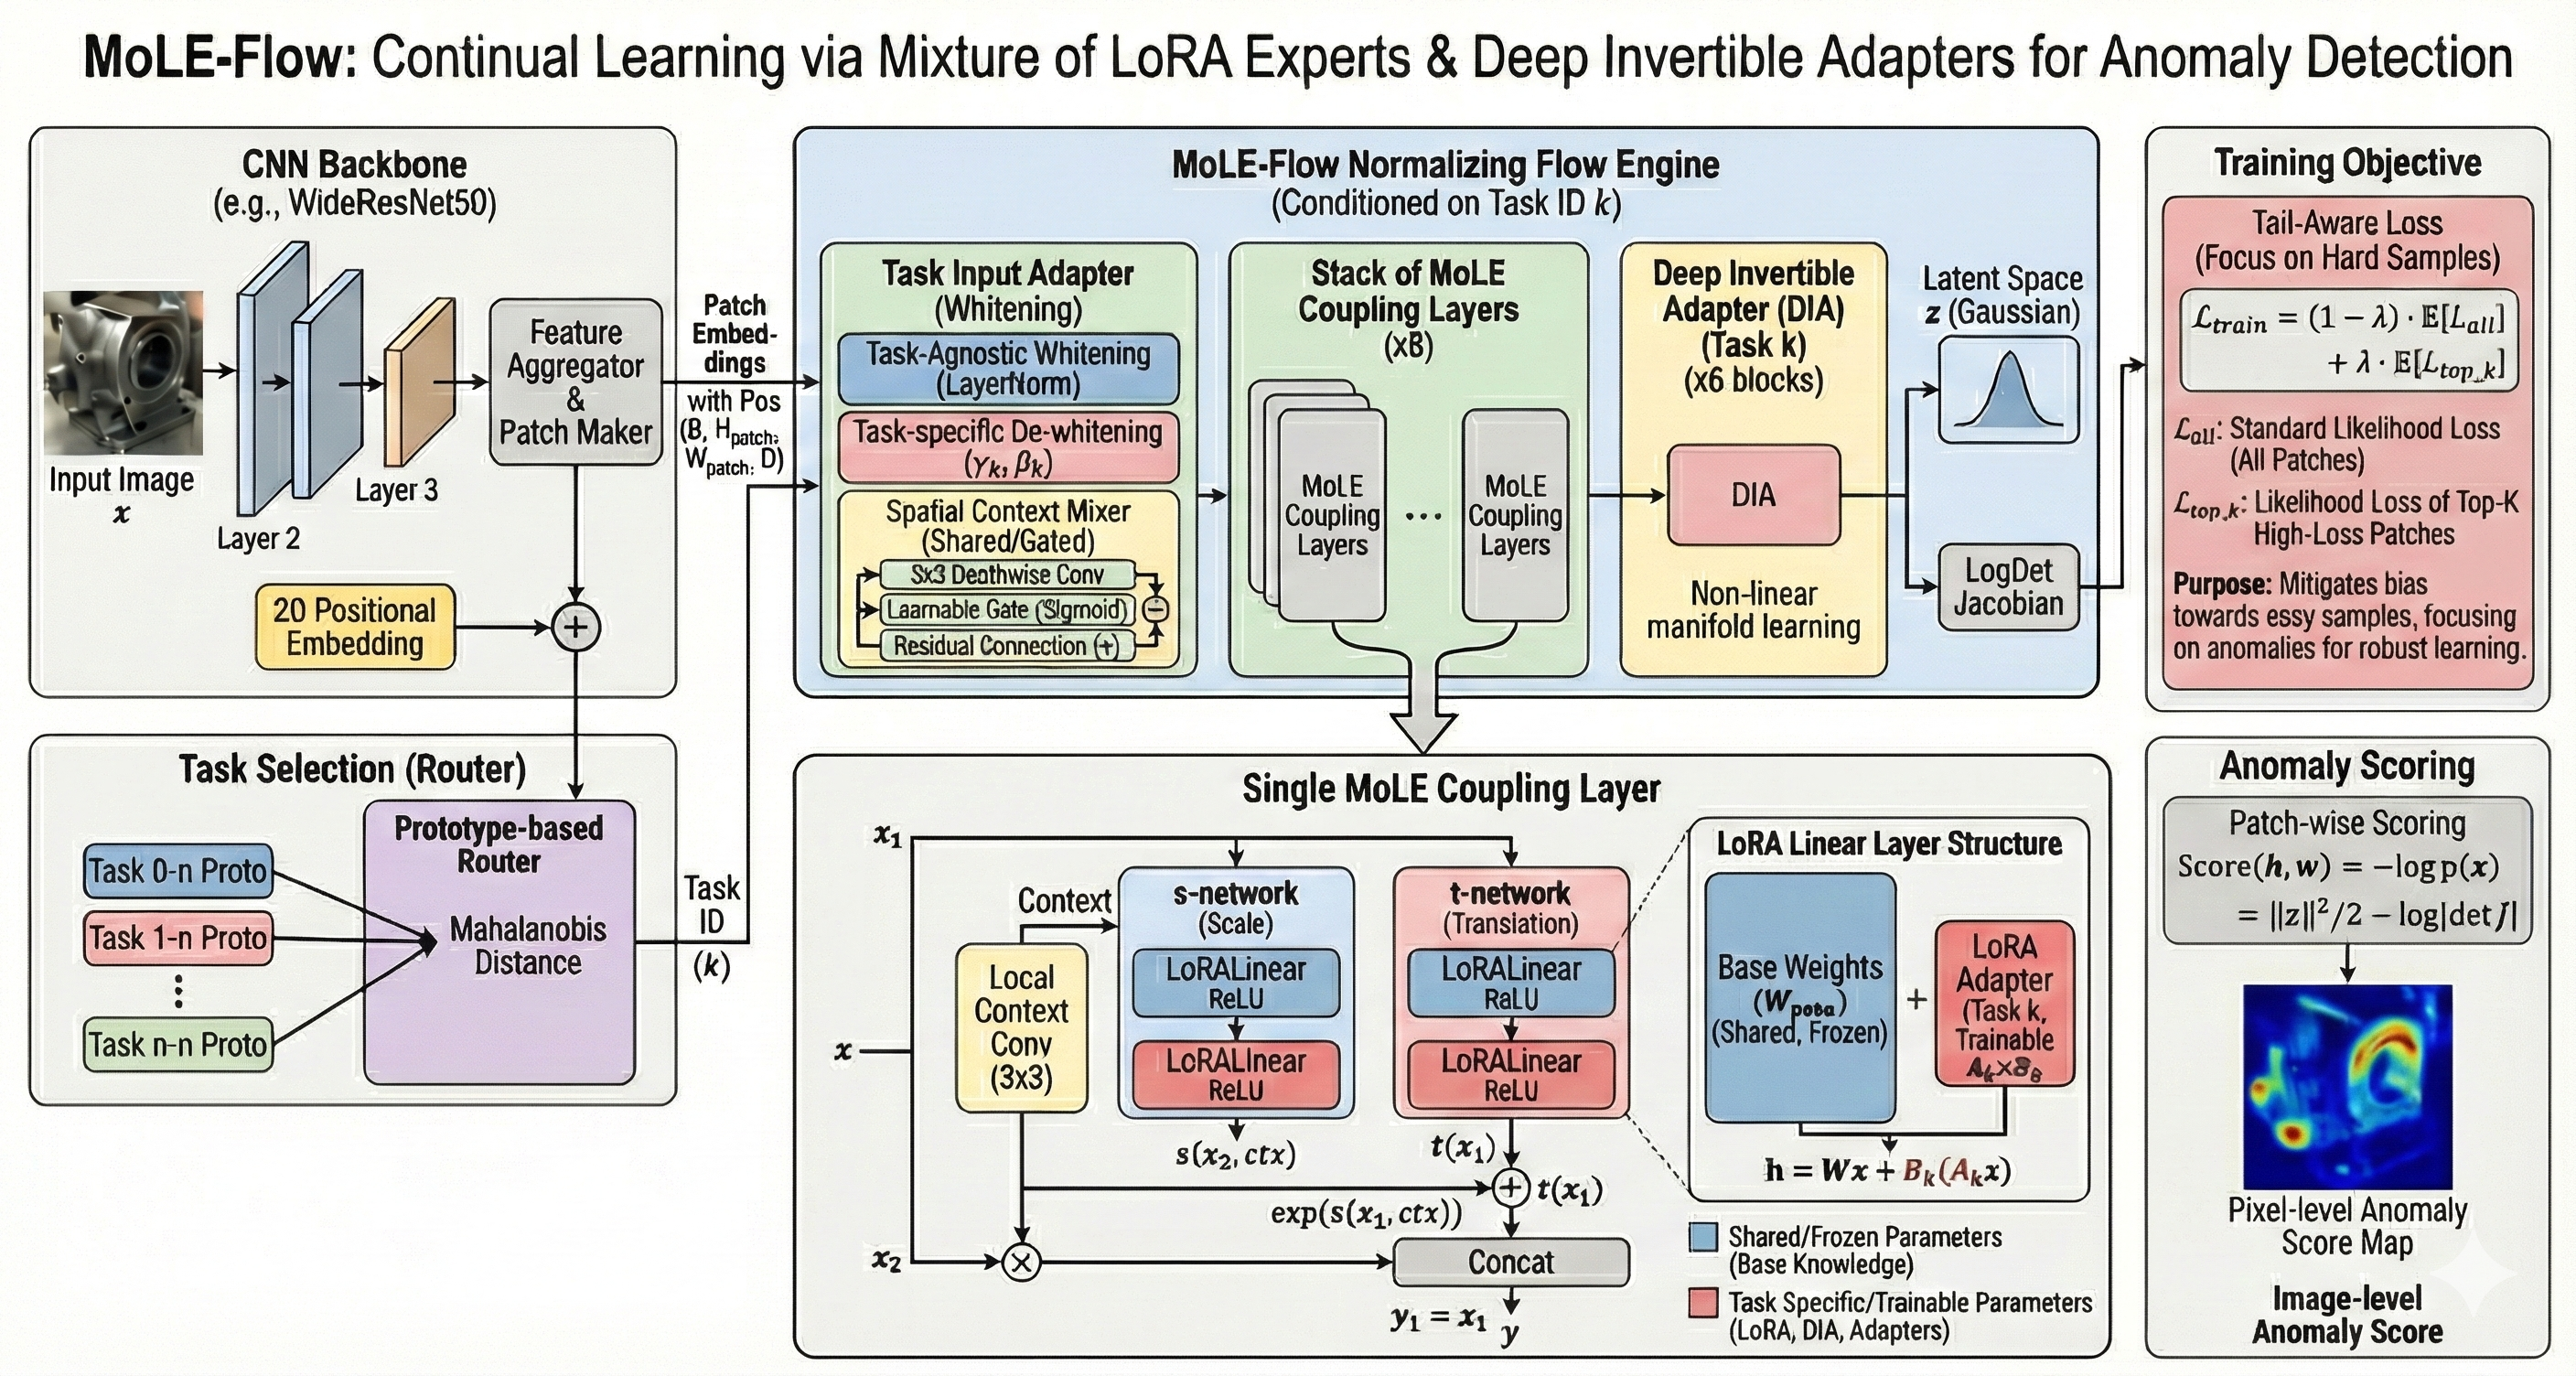
\includegraphics[width=0.98\textwidth]{figures/main2.png}
\end{center}
\end{frame}

\begin{frame}{Pipeline 수식}
\begin{equation*}
\mathbf{x} \xrightarrow{\text{Backbone}} \mathbf{F} \xrightarrow{\text{PE}} \mathbf{F}' \xrightarrow{\text{Whitening}} \hat{\mathbf{F}} \xrightarrow{\text{SCM}} \tilde{\mathbf{F}} \xrightarrow{\text{NF+LoRA}} \mathbf{z}' \xrightarrow{\text{DIA}} (\mathbf{z}, \log|\det \mathbf{J}|)
\end{equation*}

\vspace{1em}
\begin{columns}
\begin{column}{0.5\textwidth}
\textbf{공유/고정 파라미터}
\begin{itemize}
    \item Backbone (ViT-Base)
    \item Base NF weights ($\mathbf{W}_{\text{base}}$)
    \item Spatial Context Mixer
\end{itemize}
\end{column}

\begin{column}{0.5\textwidth}
\textbf{Task-specific 파라미터}
\begin{itemize}
    \item LoRA: $\mathbf{A}_t, \mathbf{B}_t$
    \item Whitening: $\gamma_t, \beta_t$
    \item DIA: 별도 flow 블록
\end{itemize}
\end{column}
\end{columns}

\vspace{1em}
\begin{alertblock}{핵심 장점}
작업당 \textbf{약 10.8\%}의 추가 파라미터만으로 완전한 작업 분리 달성
\end{alertblock}
\end{frame}

%===============================================================================
\section{Feature Extraction}
%===============================================================================

\begin{frame}{Feature Extraction \& Preprocessing}
\begin{columns}
\begin{column}{0.6\textwidth}
\textbf{1. Backbone (ViT-Base)}
\begin{itemize}
    \item 사전 학습된 ViT 사용 (Frozen)
    \item 다중 스케일 특징: 블록 $\{1, 3, 5, 11\}$
\end{itemize}

\vspace{0.5em}
\textbf{2. Patch Maker}
\begin{itemize}
    \item 특징 맵을 패치 단위로 분할
    \item 출력: $\mathbf{F} \in \mathbb{R}^{B \times H \times W \times D}$
\end{itemize}

\vspace{0.5em}
\textbf{3. Positional Encoding}
\begin{itemize}
    \item NF의 순열 불변성 극복
    \item 2D Sinusoidal PE 추가
\end{itemize}
\begin{equation*}
\mathbf{F}' = \mathbf{F} + \mathbf{P}
\end{equation*}
\end{column}

\begin{column}{0.4\textwidth}
\centering
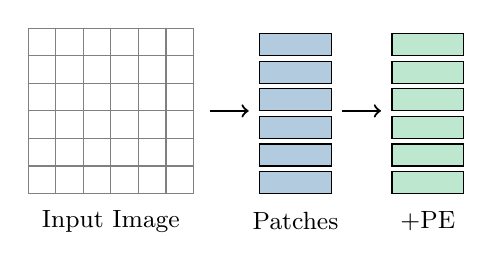
\begin{tikzpicture}[scale=0.7]
    % Image grid
    \draw[step=0.5cm, gray, thin] (0,0) grid (3,3);
    \node at (1.5,-0.5) {\small Input Image};

    % Arrow
    \draw[->, thick] (3.3,1.5) -- (4,1.5);

    % Patch embeddings
    \foreach \y in {0,0.5,1,1.5,2,2.5} {
        \draw[fill=mainblue!30] (4.2,\y) rectangle (5.5,\y+0.4);
    }
    \node at (4.85,-0.5) {\small Patches};

    % Arrow
    \draw[->, thick] (5.7,1.5) -- (6.4,1.5);

    % PE added
    \foreach \y in {0,0.5,1,1.5,2,2.5} {
        \draw[fill=accentgreen!30] (6.6,\y) rectangle (7.9,\y+0.4);
    }
    \node at (7.25,-0.5) {\small +PE};
\end{tikzpicture}
\end{column}
\end{columns}
\end{frame}

%===============================================================================
\section{Task Adapters}
%===============================================================================

\begin{frame}{Task Adapters: Whitening}
\textbf{문제: 작업 간 특징 분포 차이}
\begin{itemize}
    \item Task 0 이후 Base Flow는 동결됨
    \item 새로운 작업의 분포가 다르면 성능 저하
\end{itemize}

\vspace{1em}
\textbf{해결: 2단계 Whitening 전략}

\begin{columns}
\begin{column}{0.5\textwidth}
\textbf{Step 1: Task-Agnostic Whitening}
\begin{equation*}
\mathbf{x}_{\text{white}} = \frac{\mathbf{F}' - \mathbb{E}[\mathbf{F}']}{\sqrt{\text{Var}[\mathbf{F}'] + \epsilon}}
\end{equation*}
\begin{itemize}
    \item 모든 작업을 동일한 시작점으로
    \item 학습 파라미터 없음
\end{itemize}
\end{column}

\begin{column}{0.5\textwidth}
\textbf{Step 2: Task-Specific De-whitening}
\begin{align*}
\gamma_t &\in [0.5, 2.0] \\
\beta_t &\in [-2.0, 2.0] \\
\hat{\mathbf{F}}_t &= \gamma_t \odot \mathbf{x}_{\text{white}} + \beta_t
\end{align*}
\begin{itemize}
    \item 작업별 학습 파라미터
    \item 범위 제한으로 안정성 확보
\end{itemize}
\end{column}
\end{columns}
\end{frame}

%===============================================================================
\section{MoLE-Flow}
%===============================================================================

\begin{frame}{MoLE-Flow: Spatial Context Mixer}
\textbf{문제: 패치 독립 처리의 한계}
\begin{itemize}
    \item 기존 NF는 패치를 독립적으로 처리
    \item 주변 패치와의 관계 정보 부족
\end{itemize}

\vspace{1em}
\textbf{해결: Spatial Context Mixer}
\begin{align*}
\mathbf{x}_{\text{context}} &= \text{DepthwiseConv}_{3 \times 3}(\mathbf{x}) \\
g &= \sigma(\theta_{\text{gate}}) \\
\mathbf{x}_{\text{mixed}} &= (1 - g) \cdot \mathbf{x} + g \cdot \mathbf{x}_{\text{context}}
\end{align*}

\begin{block}{효과}
주변 문맥과의 \textbf{상대적 불일치}를 명시적으로 파악 $\rightarrow$ 국소적 이상 탐지에 필수적인 \textbf{Spatial Inductive Bias} 제공
\end{block}
\end{frame}

\begin{frame}{MoLE-Flow: LoRA-based Coupling Layer}
\begin{center}
\includegraphics[width=0.85\textwidth]{Molesubnet.png}
\end{center}

\vspace{0.5em}
\textbf{LoRALinear 구조:}
$\mathbf{h}(\mathbf{x}) = \underbrace{\mathbf{W}_{\text{base}}\mathbf{x}}_{\text{Base (Frozen)}} + \underbrace{\frac{\alpha}{r}(\mathbf{B}\mathbf{A})\mathbf{x}}_{\text{LoRA (Task-specific)}} + (\mathbf{b}_{\text{base}} + \mathbf{b}_t)$
\end{frame}

\begin{frame}{MoLE-Flow: LoRA-based Coupling Layer (상세)}
\begin{columns}
\begin{column}{0.5\textwidth}
\textbf{Base Linear (Frozen Anchor)}
\begin{itemize}
    \item Task 0에서 학습 후 고정
    \item 범용적인 특징 변환 역할
    \item 모든 작업이 공유
\end{itemize}
\end{column}

\begin{column}{0.5\textwidth}
\textbf{LoRA Linear (Task-Specialist)}
\begin{itemize}
    \item 작업 고유 분포 특성 보정
    \item 저랭크 행렬 ($r=64$)
    \item 작업마다 새로운 $\mathbf{A}, \mathbf{B}$ 생성
\end{itemize}
\end{column}
\end{columns}

\vspace{1em}
\begin{alertblock}{파라미터 효율성}
전체 대비 \textbf{약 8.3\%}의 파라미터만으로 효과적인 작업 적응
\end{alertblock}
\end{frame}

\begin{frame}{MoLE-Flow: Context-Aware s/t Networks}
\textbf{Coupling Layer 변환: $\mathbf{y}_2 = \mathbf{x}_2 \odot \exp(\mathbf{s}) + \mathbf{t}$}

\vspace{1em}
\begin{columns}
\begin{column}{0.5\textwidth}
\textbf{Scale Network (Context-Aware)}
\begin{equation*}
\mathbf{s} = f_s([\mathbf{x}; \mathbf{ctx}])
\end{equation*}
\begin{itemize}
    \item 원본 + 문맥 정보 결합
    \item 스케일 변화는 주변과의 상호작용에 민감
\end{itemize}
\end{column}

\begin{column}{0.5\textwidth}
\textbf{Translation Network (Context-Free)}
\begin{equation*}
\mathbf{t} = f_t(\mathbf{x})
\end{equation*}
\begin{itemize}
    \item 원본 특징만 사용
    \item 분포 중심은 패치 고유 특성에 종속
\end{itemize}
\end{column}
\end{columns}

\vspace{1em}
\begin{block}{설계 철학}
$\mathbf{s}$와 $\mathbf{t}$의 역할 분리 $\rightarrow$ 각각에 적합한 inductive bias 반영
\end{block}
\end{frame}

\begin{frame}{MoLE-Flow: Deep Invertible Adapter (DIA)}
\textbf{문제: 선형 LoRA의 한계}
\begin{itemize}
    \item LoRA, Whitening은 선형 변환
    \item 복잡한 비선형 분포 차이 보상 어려움
\end{itemize}

\vspace{1em}
\textbf{해결: DIA (비선형 가역 적응)}
\begin{equation*}
\mathbf{z}_{\text{final}} = f_{\text{DIA}}^{(t)}(\mathbf{z}_{\text{base}})
\end{equation*}

\vspace{0.5em}
\textbf{DIA의 장점:}
\begin{enumerate}
    \item \textbf{비선형 매니폴드 적응}: 선형 LoRA가 표현 불가능한 변환 학습
    \item \textbf{가역성 보장}: 밀도 추정 속성 유지
    \item \textbf{완전한 작업 분리}: 작업별 독립 파라미터
    \item \textbf{후처리 위치}: Base NF 출력에 추가 보정
\end{enumerate}
\end{frame}

%===============================================================================
\section{Training \& Inference}
%===============================================================================

\begin{frame}{Training Objective: Likelihood Calculation}
\textbf{Normalizing Flow의 핵심: 변수 변환}
\begin{equation*}
\log p(\mathbf{x}) = \log p(\mathbf{z}_{\text{final}}) + \log|\det \mathbf{J}_{\text{total}}|
\end{equation*}

\vspace{1em}
\begin{columns}
\begin{column}{0.5\textwidth}
\textbf{잠재 확률}
\begin{equation*}
\log p(\mathbf{z}) = -\frac{1}{2}\|\mathbf{z}\|_2^2 - \frac{D}{2}\log(2\pi)
\end{equation*}
\begin{itemize}
    \item 표준 정규분포 가정
    \item 원점에 가까울수록 높은 확률
\end{itemize}
\end{column}

\begin{column}{0.5\textwidth}
\textbf{Jacobian 누적}
\begin{equation*}
\log|\det \mathbf{J}_{\text{total}}| = \log|\det \mathbf{J}_{\text{flow}}| + \log|\det \mathbf{J}_{\text{DIA}}|
\end{equation*}
\begin{itemize}
    \item 각 변환의 부피 변화율
    \item 밀도 보정 역할
\end{itemize}
\end{column}
\end{columns}
\end{frame}

\begin{frame}{Training Objective: Tail-Aware Loss}
\textbf{문제: 일반 NLL의 한계}
\begin{itemize}
    \item 모든 패치의 평균 우도 최대화
    \item ``쉬운'' 정상 패치에만 집중 $\rightarrow$ 경계 학습 부족
\end{itemize}

\vspace{1em}
\textbf{해결: Tail-Aware Loss}
\begin{equation*}
\mathcal{L}_{\text{train}} = (1 - \lambda) \cdot \mathbb{E}[\mathcal{L}_{\text{all}}] + \lambda \cdot \mathbb{E}[\mathcal{L}_{\text{top-k}}]
\end{equation*}

\begin{itemize}
    \item $\lambda = 0.5$: 가중치 비율 (최적화된 값)
    \item $\mathcal{L}_{\text{top-k}}$: 상위 5\% 고손실 패치의 평균 NLL
\end{itemize}

\begin{block}{효과}
정상 분포의 \textbf{경계(Boundary)}를 더 명확하게 학습
\end{block}
\end{frame}

\begin{frame}{Inference: Task Routing}
\textbf{핵심 문제: 추론 시 Task ID가 주어지지 않음}

\vspace{1em}
\textbf{해결: Prototype-based Mahalanobis Router}
\begin{equation*}
t^* = \argmin_t D_M(\mathbf{f}, t), \quad D_M(\mathbf{f}, t) = \sqrt{(\mathbf{f} - \boldsymbol{\mu}_t)^\top \boldsymbol{\Sigma}_t^{-1} (\mathbf{f} - \boldsymbol{\mu}_t)}
\end{equation*}

\vspace{0.5em}
\textbf{장점:}
\begin{itemize}
    \item \textbf{One-stage}: 별도의 라우팅 추론 불필요
    \item \textbf{공분산 고려}: 분포 형태를 반영한 거리 측정
    \item \textbf{스케일 불변}: 특징 차원 간 스케일 차이 자동 보정
\end{itemize}

\begin{alertblock}{기존 방법 대비 장점}
기존: Two-stage (라우팅 $\rightarrow$ 탐지) \\
Ours: \textbf{One-stage} (라우팅 + 탐지 동시)
\end{alertblock}
\end{frame}

\begin{frame}{Inference: Anomaly Scoring}
\textbf{Step 1: Patch-wise Scoring}
\begin{equation*}
\text{Score}_{(h,w)} = \underbrace{\frac{1}{2}\|\mathbf{z}_{(h,w)}\|^2}_{\text{Distance Score}} \underbrace{- \log|\det \mathbf{J}|_{(h,w)}}_{\text{Distortion Score}}
\end{equation*}

\vspace{0.5em}
\textbf{Step 2: Top-K Mean Aggregation}
\begin{equation*}
\text{Final Score} = \frac{1}{K} \sum_{i=1}^{K} S_{\text{top}}^{(i)}
\end{equation*}

\begin{columns}
\begin{column}{0.5\textwidth}
\textbf{vs Max}
\begin{itemize}
    \item 단일 노이즈에 의한 오탐 방지
\end{itemize}
\end{column}
\begin{column}{0.5\textwidth}
\textbf{vs Mean}
\begin{itemize}
    \item 이상 신호 희석 방지
    \item 결함은 보통 군집 형성
\end{itemize}
\end{column}
\end{columns}
\end{frame}

%===============================================================================
\section{Experiments Part 1: Hyperparameter Optimization}
%===============================================================================

\begin{frame}{Hyperparameter Optimization Overview}
\begin{block}{실험 규모}
\textbf{78개 이상의 실험}을 수행하여 최적의 하이퍼파라미터 조합 탐색
\end{block}

\vspace{1em}
\textbf{Baseline 성능 (MVTec AD, WRN50-80ep):}
\begin{table}
\centering
\begin{tabular}{lcc}
\toprule
\textbf{Metric} & \textbf{Baseline} & \textbf{Target} \\
\midrule
Image AUC & 0.9796 & $\geq$ 0.98 \\
Pixel AP & 0.4640 & 0.54 - 0.60 \\
Routing Acc. & 100\% & 100\% \\
\bottomrule
\end{tabular}
\end{table}

\vspace{0.5em}
\textbf{최종 달성:}
\begin{itemize}
    \item \textcolor{accentgreen}{\textbf{Pixel AP: 0.5350}} (+15.3\% 개선)
    \item \textcolor{accentgreen}{\textbf{Image AUC: 0.9824}} (유지/향상)
\end{itemize}
\end{frame}

\begin{frame}{Individual Component Effects}
\textbf{각 하이퍼파라미터의 개별 효과 (vs Baseline 0.4640):}

\begin{table}
\centering
\scriptsize
\begin{tabular}{lccc}
\toprule
\textbf{Component} & \textbf{Pixel AP} & \textbf{Delta} & \textbf{Impact} \\
\midrule
\textcolor{red}{\textbf{LogdetReg 1e-4}} & 0.5055 & \textcolor{red}{\textbf{+4.15\%}} & \ding{72}\ding{72}\ding{72}\ding{72}\ding{72} \\
ScaleCtxK5 & 0.4870 & +2.30\% & \ding{72}\ding{72}\ding{72}\ding{72} \\
TopK5-TailW0.5 & 0.4866 & +2.26\% & \ding{72}\ding{72}\ding{72}\ding{72} \\
lr 3e-4 & 0.4718 & +0.78\% & \ding{72}\ding{72} \\
DIA6 & 0.4606 & -0.34\% & \ding{72} \\
\bottomrule
\end{tabular}
\end{table}

\vspace{1em}
\begin{alertblock}{핵심 발견}
\textbf{Log-determinant Regularization (1e-4)}이 \textbf{단일 최대 개선 효과} (+4.15\%)
\end{alertblock}
\end{frame}

\begin{frame}{Tail Weight Effect Analysis}
\textbf{TailWeight: 어려운 패치에 집중하는 정도}

\begin{table}
\centering
\begin{tabular}{cccc}
\toprule
\textbf{TailW} & \textbf{Pixel AP} & \textbf{Image AUC} & \textbf{최적 TailTopK} \\
\midrule
0.50 & 0.5221 & 0.983 & 5\% \\
0.55 & 0.5256 & 0.983 & 5\% \\
0.60 & 0.5290 & 0.983 & 3\% \\
0.65 & 0.5324 & 0.983 & 1\% \\
\textcolor{accentgreen}{\textbf{0.75}} & \textcolor{accentgreen}{\textbf{0.5449}} & 0.981 & 2\% \\
0.80 & 0.5447 & 0.981 & 3\% \\
\bottomrule
\end{tabular}
\end{table}

\vspace{0.5em}
\textbf{Trade-off 발견:}
\begin{itemize}
    \item TailW 증가 $\rightarrow$ Pixel AP 향상
    \item TailW $>$ 0.75 $\rightarrow$ Image AUC 약간 하락 (0.983 $\rightarrow$ 0.981)
\end{itemize}
\end{frame}

\begin{frame}{Optimization Journey}
\textbf{Baseline에서 최적 설정까지의 개선 과정:}

\begin{center}
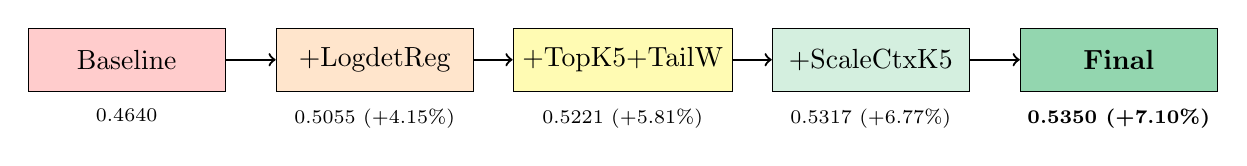
\begin{tikzpicture}[scale=0.9]
    % Baseline
    \node[draw, fill=red!20, minimum width=2.5cm, minimum height=0.8cm] (b) at (0,0) {Baseline};
    \node[below=0.1cm of b] {\scriptsize 0.4640};

    % +LogdetReg
    \node[draw, fill=orange!20, minimum width=2.5cm, minimum height=0.8cm] (l) at (3.5,0) {+LogdetReg};
    \node[below=0.1cm of l] {\scriptsize 0.5055 (+4.15\%)};

    % +TopK5+TailW
    \node[draw, fill=yellow!30, minimum width=2.5cm, minimum height=0.8cm] (t) at (7,0) {+TopK5+TailW};
    \node[below=0.1cm of t] {\scriptsize 0.5221 (+5.81\%)};

    % +ScaleCtxK5
    \node[draw, fill=accentgreen!20, minimum width=2.5cm, minimum height=0.8cm] (s) at (10.5,0) {+ScaleCtxK5};
    \node[below=0.1cm of s] {\scriptsize 0.5317 (+6.77\%)};

    % Final
    \node[draw, fill=accentgreen!50, minimum width=2.5cm, minimum height=0.8cm] (f) at (14,0) {\textbf{Final}};
    \node[below=0.1cm of f] {\scriptsize \textbf{0.5350 (+7.10\%)}};

    % Arrows
    \draw[->, thick] (b) -- (l);
    \draw[->, thick] (l) -- (t);
    \draw[->, thick] (t) -- (s);
    \draw[->, thick] (s) -- (f);
\end{tikzpicture}
\end{center}

\vspace{1em}
\textbf{최적 설정:}
\begin{itemize}
    \item \texttt{TailW=0.55, TopK=5, LogdetReg=1e-4, ScaleCtxK=5, lr=3e-4}
\end{itemize}
\end{frame}

\begin{frame}{Top 10 Experiments by Pixel AP}
\begin{table}
\centering
\scriptsize
\begin{tabular}{clccc}
\toprule
\textbf{Rank} & \textbf{Configuration} & \textbf{Image AUC} & \textbf{Pixel AP} & \textbf{Routing} \\
\midrule
1 & TailW0.55-TopK5-LogdetReg1e-4-ScaleCtxK5-lr3e-4 & 0.9824 & \textbf{0.5350} & 100\% \\
2 & TailW0.65-TailTopK3-TopK5-LogdetReg1e-4 & 0.9827 & 0.5324 & 100\% \\
3 & TopK3-TailW0.5-LogdetReg1e-4-ScaleCtxK5 & 0.9802 & 0.5317 & 100\% \\
4 & TopK5-TailW0.5-LogdetReg1e-4-ScaleCtxK5 & 0.9809 & 0.5317 & 100\% \\
5 & TailW0.6-TailTopK3-TopK5-LogdetReg1e-4-ScaleCtxK5-80ep & 0.9826 & 0.5310 & 100\% \\
6 & TailW0.6-TopK5-LogdetReg1e-4 & 0.9827 & 0.5290 & 100\% \\
7 & TailW0.55-TopK5-LogdetReg1e-4 & 0.9827 & 0.5256 & 100\% \\
8 & TailW0.5-TailTopK3-TopK5-LogdetReg1e-4 & 0.9830 & 0.5242 & 100\% \\
9 & FullBest-80ep-lr3e-4-LoRA128-C10-DIA5-TailW0.55 & \textbf{0.9836} & 0.5242 & 100\% \\
10 & TopK5-TailW0.5-LogdetReg1e-4 & 0.9826 & 0.5221 & 100\% \\
\bottomrule
\end{tabular}
\end{table}

\vspace{0.5em}
\textbf{Observation:} 모든 상위 설정에서 \textbf{Routing Accuracy 100\%} 유지
\end{frame}

\begin{frame}{Per-Class Performance Improvement}
\begin{table}
\centering
\scriptsize
\begin{tabular}{lccc}
\toprule
\textbf{Class} & \textbf{Baseline} & \textbf{Top Config} & \textbf{Improvement} \\
\midrule
carpet & 0.3601 & 0.6167 & \textcolor{accentgreen}{\textbf{+0.2566}} \\
bottle & 0.4551 & 0.6774 & \textcolor{accentgreen}{\textbf{+0.2223}} \\
leather & 0.2292 & 0.3970 & \textcolor{accentgreen}{\textbf{+0.1678}} \\
toothbrush & 0.4028 & 0.5619 & +0.1591 \\
wood & 0.3546 & 0.4453 & +0.0907 \\
hazelnut & 0.5110 & 0.5798 & +0.0688 \\
\midrule
metal\_nut & 0.8491 & 0.7776 & \textcolor{red}{-0.0715} \\
cable & 0.6575 & 0.6339 & \textcolor{red}{-0.0236} \\
\midrule
\textbf{Mean} & \textbf{0.4640} & \textbf{0.5350} & \textbf{+0.0710} \\
\bottomrule
\end{tabular}
\end{table}

\textbf{Key Observations:}
\begin{itemize}
    \item \textcolor{accentgreen}{\textbf{Textured classes}} (carpet, leather): 가장 큰 개선
    \item \textcolor{red}{\textbf{Fine-grained objects}} (metal\_nut, cable): 약간의 성능 저하
\end{itemize}
\end{frame}

\begin{frame}{Hyperparameter Sensitivity Summary}
\begin{columns}
\begin{column}{0.5\textwidth}
\textbf{DIA Blocks}
\begin{table}
\scriptsize
\begin{tabular}{ccc}
\toprule
Blocks & Image AUC & Pixel AP \\
\midrule
4 & 0.9793 & 0.4735 \\
6 & 0.9820 & 0.4606 \\
8 & \textbf{0.9825} & 0.4546 \\
\bottomrule
\end{tabular}
\end{table}
\begin{itemize}
    \item[$\uparrow$] Blocks $\rightarrow$ $\uparrow$ Image AUC
    \item[$\downarrow$] Pixel AP (trade-off)
\end{itemize}
\end{column}

\begin{column}{0.5\textwidth}
\textbf{LoRA Rank (Minimal Effect)}
\begin{table}
\scriptsize
\begin{tabular}{ccc}
\toprule
Rank & Image AUC & Pixel AP \\
\midrule
32 & 0.9794 & 0.4737 \\
64 & 0.9793 & 0.4735 \\
128 & 0.9794 & 0.4736 \\
256 & 0.9796 & 0.4741 \\
\bottomrule
\end{tabular}
\end{table}
\begin{itemize}
    \item Rank 64로 충분
    \item 파라미터 효율성 확인
\end{itemize}
\end{column}
\end{columns}

\vspace{1em}
\begin{alertblock}{Warning: Coupling Layers}
\textbf{Coupling16}: 학습 불안정 발생 (Image AUC 0.73으로 급락). 8-12 권장.
\end{alertblock}
\end{frame}

\begin{frame}{Optimal Configuration Recommendations}
\begin{columns}
\begin{column}{0.5\textwidth}
\textbf{Balanced Setting (권장)}
\begin{itemize}
    \item \texttt{tail\_weight = 0.55}
    \item \texttt{topk = 5}
    \item \texttt{logdet\_reg = 1e-4}
    \item \texttt{scale\_context\_k = 5}
    \item \texttt{lr = 3e-4}
    \item \texttt{epochs = 60}
\end{itemize}
\vspace{0.5em}
$\rightarrow$ Image AUC $\approx$ \textbf{0.982}, Pixel AP $\approx$ \textbf{0.535}
\end{column}

\begin{column}{0.5\textwidth}
\textbf{Max Image AUC Setting}
\begin{itemize}
    \item \texttt{tail\_weight = 0.55}
    \item \texttt{lora\_rank = 128}
    \item \texttt{dia\_n\_blocks = 5}
    \item \texttt{coupling = 10}
    \item \texttt{lr = 3e-4}
    \item \texttt{epochs = 80}
\end{itemize}
\vspace{0.5em}
$\rightarrow$ Image AUC $\approx$ \textbf{0.984}, Pixel AP $\approx$ \textbf{0.524}
\end{column}
\end{columns}
\end{frame}

%===============================================================================
\section{Experiments Part 2: Paper Experiment Design}
%===============================================================================

\begin{frame}{Experimental Setup}
\begin{columns}
\begin{column}{0.5\textwidth}
\textbf{Datasets}
\begin{itemize}
    \item \textbf{MVTec AD}: 15 classes, 5,354 images
    \item \textbf{VisA}: 12 classes, 10,821 images
    \item \textbf{MPDD}: 6 classes (metal parts)
\end{itemize}

\vspace{0.5em}
\textbf{Evaluation Metrics}
\begin{itemize}
    \item Image AUROC / AP (primary)
    \item Pixel AUROC / AP / PRO
    \item Forgetting (F), BWT
    \item Routing Accuracy
\end{itemize}
\end{column}

\begin{column}{0.5\textwidth}
\textbf{Implementation}
\begin{itemize}
    \item Backbone: ViT-Base-16 (frozen)
    \item NF: 8 Coupling Layers
    \item LoRA rank: 64
    \item DIA: 4 blocks
    \item Epochs: 60 per task
    \item LR: $2 \times 10^{-4}$
    \item Input: 224 $\times$ 224
\end{itemize}

\vspace{0.5em}
\textbf{Hardware}: NVIDIA RTX 4090
\end{column}
\end{columns}
\end{frame}

\begin{frame}{Continual Learning Scenarios}
\textbf{4가지 시나리오로 지속 학습 능력 검증:}

\vspace{0.5em}
\begin{enumerate}
    \item \textbf{Scenario A: Standard 5-Task Protocol}
    \begin{itemize}
        \item MVTec 15 classes $\rightarrow$ 5 tasks (각 3 classes)
        \item Task 0: leather, grid, transistor (텍스처 + 객체 혼합)
    \end{itemize}

    \vspace{0.3em}
    \item \textbf{Scenario B: Long Sequence (15-Task)}
    \begin{itemize}
        \item 15개 클래스를 각각 독립 작업으로 구성
        \item 장기 망각(Long-term Forgetting) 분석
    \end{itemize}

    \vspace{0.3em}
    \item \textbf{Scenario C: Class Order Sensitivity}
    \begin{itemize}
        \item 5개 무작위 순서로 학습
        \item Parameter Isolation의 순서 견고성 검증
    \end{itemize}

    \vspace{0.3em}
    \item \textbf{Scenario D: Task 0 Dependency Analysis}
    \begin{itemize}
        \item Texture-first vs Object-first vs Mixed-first
        \item Base weights 학습이 후속 작업에 미치는 영향
    \end{itemize}
\end{enumerate}
\end{frame}

\begin{frame}{Comparison with SOTA Methods}
\textbf{비교 대상:}

\vspace{0.5em}
\begin{columns}
\begin{column}{0.5\textwidth}
\textbf{Continual AD Methods}
\begin{itemize}
    \item \textbf{DNE}: 분포 저장 기반
    \item \textbf{UCAD}: Prompt tuning 기반 SOTA
\end{itemize}

\vspace{0.5em}
\textbf{CL + AD Adaptation}
\begin{itemize}
    \item EWC: 중요 파라미터 정규화
    \item LwF: Knowledge Distillation
    \item Replay (5\%): 데이터 저장
\end{itemize}
\end{column}

\begin{column}{0.5\textwidth}
\textbf{Bounds}
\begin{itemize}
    \item \textbf{Joint Training}: Upper bound
    \item \textbf{Task-Separated}: 망각 없음, 비효율
    \item \textbf{Fine-tuning}: Lower bound
\end{itemize}

\vspace{0.5em}
\textbf{검증 목표:}
\begin{itemize}
    \item 이상 탐지 성능 우수성
    \item Forgetting $\approx$ 0 (Parameter Isolation)
    \item Routing Accuracy 100\%
\end{itemize}
\end{column}
\end{columns}
\end{frame}

\begin{frame}{Ablation Study Design (7 Components)}
\begin{table}
\centering
\scriptsize
\begin{tabular}{lcccc}
\toprule
\textbf{Removed Component} & \textbf{Config Flag} & \textbf{$\Delta$ Img AUC} & \textbf{$\Delta$ Pix AP} & \textbf{Importance} \\
\midrule
\multicolumn{5}{l}{\textit{Core Adapters}} \\
\quad w/o DIA & \texttt{use\_dia=False} & \textcolor{red}{-3.14\%} & -1.49\% & \ding{72}\ding{72}\ding{72}\ding{72}\ding{72} \\
\quad w/o Whitening & \texttt{use\_task\_adapter=False} & \textcolor{red}{-1.89\%} & -2.74\% & \ding{72}\ding{72}\ding{72}\ding{72} \\
\quad w/o LoRA & \texttt{use\_lora=False} & +0.04\% & +0.18\% & \ding{72} \\
\midrule
\multicolumn{5}{l}{\textit{Context Modules}} \\
\quad w/o Spatial Context & & -0.21\% & -0.76\% & \ding{72}\ding{72} \\
\quad w/o Scale Context & & -0.18\% & -0.41\% & \ding{72}\ding{72} \\
\midrule
\multicolumn{5}{l}{\textit{Loss Components}} \\
\quad w/o Tail-Aware Loss & & - & - & \ding{72}\ding{72}\ding{72} \\
\quad w/o LogdetReg & \texttt{logdet\_reg=0} & - & \textcolor{red}{-4.15\%} & \ding{72}\ding{72}\ding{72}\ding{72}\ding{72} \\
\bottomrule
\end{tabular}
\end{table}

\begin{alertblock}{Key Insight}
\textbf{DIA}가 Image AUC에, \textbf{LogdetReg}가 Pixel AP에 가장 중요
\end{alertblock}
\end{frame}

\begin{frame}{Cross-Dataset Generalization}
\textbf{MVTec $\rightarrow$ VisA $\rightarrow$ MPDD 일반화 평가:}

\begin{table}
\centering
\begin{tabular}{lcccc}
\toprule
\textbf{Dataset} & \textbf{Classes} & \textbf{Image AUC} & \textbf{Pixel AP} & \textbf{Routing Acc.} \\
\midrule
MVTec AD & 15 & \textbf{0.9824} & \textbf{0.5350} & 100\% \\
VisA & 12 & 0.8566 & 0.2878 & 100\% \\
MPDD & 6 & 0.9019 & 0.2890 & 98.12\% \\
\bottomrule
\end{tabular}
\end{table}

\vspace{0.5em}
\textbf{VisA Analysis:}
\begin{itemize}
    \item 복잡한 텍스처와 미세 결함 $\rightarrow$ 더 도전적
    \item 병목 클래스: macaroni1/2 (Pixel AP $<$ 0.1)
    \item ViT backbone: Image AUC 0.88 (WRN50 대비 +4.2\%)
\end{itemize}

\textbf{MPDD:}
\begin{itemize}
    \item 금속 표면의 유사성 $\rightarrow$ Routing 오류 (98.12\%)
\end{itemize}
\end{frame}

\begin{frame}{Continual Learning Analysis}
\textbf{Forgetting 분석:}
\begin{itemize}
    \item Parameter Isolation (LoRA + DIA) $\rightarrow$ \textbf{Forgetting $\approx$ 0}
    \item vs Fine-tuning: 급격한 성능 하락
    \item vs EWC/LwF: 완만한 하락
\end{itemize}

\vspace{1em}
\textbf{Router Performance:}
\begin{itemize}
    \item 5-Task: 100\% Routing Accuracy
    \item 15-Task: Oracle과의 Gap 분석
    \item Task 수 증가에 따른 Scalability 검증
\end{itemize}

\vspace{1em}
\textbf{Storage Efficiency:}
\begin{itemize}
    \item MoLE-Flow: 약 2MB/Task (LoRA + DIA)
    \item vs Replay (5\%): 50MB/Task $\rightarrow$ \textbf{25x 절약}
\end{itemize}
\end{frame}

%===============================================================================
\section{Conclusion \& Future Work}
%===============================================================================

\begin{frame}{Summary}
\textbf{MoLE-Flow: 지속적 이상 탐지를 위한 프레임워크}

\vspace{1em}
\begin{enumerate}
    \item \textbf{Parameter Isolation}: Base 공유 + Task-specific 어댑터
    \item \textbf{MoLE}: LoRA 기반 경량 작업 적응
    \item \textbf{WhiteningAdapter}: 분포 정렬을 통한 안정적 학습
    \item \textbf{DIA}: 비선형 매니폴드 적응
    \item \textbf{Prototype Router}: One-stage 추론
    \item \textbf{Tail-Aware Loss}: 경계 학습 강화
\end{enumerate}

\vspace{1em}
\begin{block}{핵심 장점}
\begin{itemize}
    \item 파멸적 망각 방지 (Forgetting $\approx$ 0)
    \item 파라미터 효율성 (작업당 $\sim$10.8\%)
    \item Task ID 없이 추론 가능 (Routing 100\%)
\end{itemize}
\end{block}
\end{frame}

\begin{frame}{Key Results}
\begin{columns}
\begin{column}{0.5\textwidth}
\textbf{MVTec AD (Best Performance)}
\begin{itemize}
    \item Image AUC: \textbf{0.9836}
    \item Pixel AP: \textbf{0.5350}
    \item Routing Acc.: \textbf{100\%}
\end{itemize}

\vspace{1em}
\textbf{개선 효과}
\begin{itemize}
    \item Pixel AP: +15.3\% (Baseline 대비)
    \item 78개 실험을 통한 최적화
\end{itemize}
\end{column}

\begin{column}{0.5\textwidth}
\textbf{Cross-Dataset}
\begin{itemize}
    \item VisA: Image AUC 0.8566
    \item MPDD: Image AUC 0.9019
\end{itemize}

\vspace{1em}
\textbf{핵심 하이퍼파라미터}
\begin{itemize}
    \item LogdetReg 1e-4 (최대 효과)
    \item TailW 0.55-0.75
    \item ScaleCtxK 5
\end{itemize}
\end{column}
\end{columns}
\end{frame}

\begin{frame}{Future Work}
\textbf{1. 성능 향상 방향}
\begin{itemize}
    \item Pixel AP 0.6+ 달성을 위한 추가 최적화
    \item 고해상도 입력 (448 $\times$ 448) 적용
    \item DINOv2 ViT-L/H 등 강력한 backbone 탐색
\end{itemize}

\vspace{1em}
\textbf{2. 일반화 강화}
\begin{itemize}
    \item VisA 병목 클래스 (macaroni) 특화 전략
    \item Multi-scale 평가 앙상블
    \item Class-specific hyperparameter tuning
\end{itemize}

\vspace{1em}
\textbf{3. 실용화 연구}
\begin{itemize}
    \item 실시간 추론 최적화
    \item 경량화 (Quantization, Pruning)
    \item 온라인 학습 시나리오 확장
\end{itemize}
\end{frame}

\begin{frame}
\centering
\Huge Thank You!

\vspace{2em}
\Large Questions?

\vspace{3em}
\normalsize
\textbf{GitHub}: \texttt{github.com/your-repo/moleflow}

\textbf{Contact}: author@example.com
\end{frame}

\end{document}
